\documentclass[twoside]{book}

% Packages required by doxygen
\usepackage{fixltx2e}
\usepackage{calc}
\usepackage{doxygen}
\usepackage[export]{adjustbox} % also loads graphicx
\usepackage{graphicx}
\usepackage[utf8]{inputenc}
\usepackage{makeidx}
\usepackage{multicol}
\usepackage{multirow}
\PassOptionsToPackage{warn}{textcomp}
\usepackage{textcomp}
\usepackage[nointegrals]{wasysym}
\usepackage[table]{xcolor}

% Font selection
\usepackage[T1]{fontenc}
\usepackage[scaled=.90]{helvet}
\usepackage{courier}
\usepackage{amssymb}
\usepackage{sectsty}
\renewcommand{\familydefault}{\sfdefault}
\allsectionsfont{%
  \fontseries{bc}\selectfont%
  \color{darkgray}%
}
\renewcommand{\DoxyLabelFont}{%
  \fontseries{bc}\selectfont%
  \color{darkgray}%
}
\newcommand{\+}{\discretionary{\mbox{\scriptsize$\hookleftarrow$}}{}{}}

% Page & text layout
\usepackage{geometry}
\geometry{%
  a4paper,%
  top=2.5cm,%
  bottom=2.5cm,%
  left=2.5cm,%
  right=2.5cm%
}
\tolerance=750
\hfuzz=15pt
\hbadness=750
\setlength{\emergencystretch}{15pt}
\setlength{\parindent}{0cm}
\setlength{\parskip}{3ex plus 2ex minus 2ex}
\makeatletter
\renewcommand{\paragraph}{%
  \@startsection{paragraph}{4}{0ex}{-1.0ex}{1.0ex}{%
    \normalfont\normalsize\bfseries\SS@parafont%
  }%
}
\renewcommand{\subparagraph}{%
  \@startsection{subparagraph}{5}{0ex}{-1.0ex}{1.0ex}{%
    \normalfont\normalsize\bfseries\SS@subparafont%
  }%
}
\makeatother

% Headers & footers
\usepackage{fancyhdr}
\pagestyle{fancyplain}
\fancyhead[LE]{\fancyplain{}{\bfseries\thepage}}
\fancyhead[CE]{\fancyplain{}{}}
\fancyhead[RE]{\fancyplain{}{\bfseries\leftmark}}
\fancyhead[LO]{\fancyplain{}{\bfseries\rightmark}}
\fancyhead[CO]{\fancyplain{}{}}
\fancyhead[RO]{\fancyplain{}{\bfseries\thepage}}
\fancyfoot[LE]{\fancyplain{}{}}
\fancyfoot[CE]{\fancyplain{}{}}
\fancyfoot[RE]{\fancyplain{}{\bfseries\scriptsize Generated by Doxygen }}
\fancyfoot[LO]{\fancyplain{}{\bfseries\scriptsize Generated by Doxygen }}
\fancyfoot[CO]{\fancyplain{}{}}
\fancyfoot[RO]{\fancyplain{}{}}
\renewcommand{\footrulewidth}{0.4pt}
\renewcommand{\chaptermark}[1]{%
  \markboth{#1}{}%
}
\renewcommand{\sectionmark}[1]{%
  \markright{\thesection\ #1}%
}

% Indices & bibliography
\usepackage{natbib}
\usepackage[titles]{tocloft}
\setcounter{tocdepth}{3}
\setcounter{secnumdepth}{5}
\makeindex

% Hyperlinks (required, but should be loaded last)
\usepackage{ifpdf}
\ifpdf
  \usepackage[pdftex,pagebackref=true]{hyperref}
\else
  \usepackage[ps2pdf,pagebackref=true]{hyperref}
\fi
\hypersetup{%
  colorlinks=true,%
  linkcolor=blue,%
  citecolor=blue,%
  unicode%
}

% Custom commands
\newcommand{\clearemptydoublepage}{%
  \newpage{\pagestyle{empty}\cleardoublepage}%
}

\usepackage{caption}
\captionsetup{labelsep=space,justification=centering,font={bf},singlelinecheck=off,skip=4pt,position=top}

%===== C O N T E N T S =====

\begin{document}

% Titlepage & ToC
\hypersetup{pageanchor=false,
             bookmarksnumbered=true,
             pdfencoding=unicode
            }
\pagenumbering{alph}
\begin{titlepage}
\vspace*{7cm}
\begin{center}%
{\Large My Project }\\
\vspace*{1cm}
{\large Generated by Doxygen 1.8.14}\\
\end{center}
\end{titlepage}
\clearemptydoublepage
\pagenumbering{roman}
\tableofcontents
\clearemptydoublepage
\pagenumbering{arabic}
\hypersetup{pageanchor=true}

%--- Begin generated contents ---
\chapter{Hierarchical Index}
\section{Class Hierarchy}
This inheritance list is sorted roughly, but not completely, alphabetically\+:\begin{DoxyCompactList}
\item \contentsline{section}{Tests.\+Bishop\+Test}{\pageref{class_tests_1_1_bishop_test}}{}
\item \contentsline{section}{Tests.\+Board\+Test}{\pageref{class_tests_1_1_board_test}}{}
\item \contentsline{section}{Source\+Files.\+Coordinate}{\pageref{class_source_files_1_1_coordinate}}{}
\item \contentsline{section}{Source\+Files.\+Field}{\pageref{class_source_files_1_1_field}}{}
\item \contentsline{section}{Source\+Files.\+Global\+Constants}{\pageref{class_source_files_1_1_global_constants}}{}
\begin{DoxyCompactList}
\item \contentsline{section}{Source\+Files.\+Board}{\pageref{class_source_files_1_1_board}}{}
\end{DoxyCompactList}
\item J\+Frame\begin{DoxyCompactList}
\item \contentsline{section}{G\+U\+I.\+G\+U\+I\+Main}{\pageref{class_g_u_i_1_1_g_u_i_main}}{}
\item \contentsline{section}{Tests.\+Polygon\+Test}{\pageref{class_tests_1_1_polygon_test}}{}
\end{DoxyCompactList}
\item \contentsline{section}{Tests.\+King\+Test}{\pageref{class_tests_1_1_king_test}}{}
\item \contentsline{section}{Tests.\+Knight\+Tests}{\pageref{class_tests_1_1_knight_tests}}{}
\item \contentsline{section}{Source\+Files.\+Move\+Record}{\pageref{class_source_files_1_1_move_record}}{}
\item \contentsline{section}{Tests.\+Pawn\+Tests}{\pageref{class_tests_1_1_pawn_tests}}{}
\item \contentsline{section}{Source\+Files.\+Piece}{\pageref{class_source_files_1_1_piece}}{}
\begin{DoxyCompactList}
\item \contentsline{section}{Source\+Files.\+Bishop}{\pageref{class_source_files_1_1_bishop}}{}
\item \contentsline{section}{Source\+Files.\+King}{\pageref{class_source_files_1_1_king}}{}
\item \contentsline{section}{Source\+Files.\+Knight}{\pageref{class_source_files_1_1_knight}}{}
\item \contentsline{section}{Source\+Files.\+Pawn}{\pageref{class_source_files_1_1_pawn}}{}
\item \contentsline{section}{Source\+Files.\+Queen}{\pageref{class_source_files_1_1_queen}}{}
\item \contentsline{section}{Source\+Files.\+Rook}{\pageref{class_source_files_1_1_rook}}{}
\end{DoxyCompactList}
\item \contentsline{section}{Tests.\+Queen\+Test}{\pageref{class_tests_1_1_queen_test}}{}
\item \contentsline{section}{Tests.\+Rook\+Test}{\pageref{class_tests_1_1_rook_test}}{}
\item Polygon\begin{DoxyCompactList}
\item \contentsline{section}{G\+U\+I.\+Colored\+Polygon}{\pageref{class_g_u_i_1_1_colored_polygon}}{}
\end{DoxyCompactList}
\end{DoxyCompactList}

\chapter{Class Index}
\section{Class List}
Here are the classes, structs, unions and interfaces with brief descriptions\+:\begin{DoxyCompactList}
\item\contentsline{section}{\mbox{\hyperlink{class_source_files_1_1_bishop}{Source\+Files.\+Bishop}} }{\pageref{class_source_files_1_1_bishop}}{}
\item\contentsline{section}{\mbox{\hyperlink{class_tests_1_1_bishop_test}{Tests.\+Bishop\+Test}} }{\pageref{class_tests_1_1_bishop_test}}{}
\item\contentsline{section}{\mbox{\hyperlink{class_source_files_1_1_board}{Source\+Files.\+Board}} }{\pageref{class_source_files_1_1_board}}{}
\item\contentsline{section}{\mbox{\hyperlink{class_tests_1_1_board_test}{Tests.\+Board\+Test}} }{\pageref{class_tests_1_1_board_test}}{}
\item\contentsline{section}{\mbox{\hyperlink{class_g_u_i_1_1_colored_polygon}{G\+U\+I.\+Colored\+Polygon}} }{\pageref{class_g_u_i_1_1_colored_polygon}}{}
\item\contentsline{section}{\mbox{\hyperlink{class_source_files_1_1_coordinate}{Source\+Files.\+Coordinate}} }{\pageref{class_source_files_1_1_coordinate}}{}
\item\contentsline{section}{\mbox{\hyperlink{class_source_files_1_1_field}{Source\+Files.\+Field}} }{\pageref{class_source_files_1_1_field}}{}
\item\contentsline{section}{\mbox{\hyperlink{class_source_files_1_1_global_constants}{Source\+Files.\+Global\+Constants}} }{\pageref{class_source_files_1_1_global_constants}}{}
\item\contentsline{section}{\mbox{\hyperlink{class_g_u_i_1_1_g_u_i_main}{G\+U\+I.\+G\+U\+I\+Main}} }{\pageref{class_g_u_i_1_1_g_u_i_main}}{}
\item\contentsline{section}{\mbox{\hyperlink{class_source_files_1_1_king}{Source\+Files.\+King}} }{\pageref{class_source_files_1_1_king}}{}
\item\contentsline{section}{\mbox{\hyperlink{class_tests_1_1_king_test}{Tests.\+King\+Test}} }{\pageref{class_tests_1_1_king_test}}{}
\item\contentsline{section}{\mbox{\hyperlink{class_source_files_1_1_knight}{Source\+Files.\+Knight}} }{\pageref{class_source_files_1_1_knight}}{}
\item\contentsline{section}{\mbox{\hyperlink{class_tests_1_1_knight_tests}{Tests.\+Knight\+Tests}} }{\pageref{class_tests_1_1_knight_tests}}{}
\item\contentsline{section}{\mbox{\hyperlink{class_source_files_1_1_move_record}{Source\+Files.\+Move\+Record}} }{\pageref{class_source_files_1_1_move_record}}{}
\item\contentsline{section}{\mbox{\hyperlink{class_source_files_1_1_pawn}{Source\+Files.\+Pawn}} }{\pageref{class_source_files_1_1_pawn}}{}
\item\contentsline{section}{\mbox{\hyperlink{class_tests_1_1_pawn_tests}{Tests.\+Pawn\+Tests}} }{\pageref{class_tests_1_1_pawn_tests}}{}
\item\contentsline{section}{\mbox{\hyperlink{class_source_files_1_1_piece}{Source\+Files.\+Piece}} }{\pageref{class_source_files_1_1_piece}}{}
\item\contentsline{section}{\mbox{\hyperlink{class_tests_1_1_polygon_test}{Tests.\+Polygon\+Test}} }{\pageref{class_tests_1_1_polygon_test}}{}
\item\contentsline{section}{\mbox{\hyperlink{class_source_files_1_1_queen}{Source\+Files.\+Queen}} }{\pageref{class_source_files_1_1_queen}}{}
\item\contentsline{section}{\mbox{\hyperlink{class_tests_1_1_queen_test}{Tests.\+Queen\+Test}} }{\pageref{class_tests_1_1_queen_test}}{}
\item\contentsline{section}{\mbox{\hyperlink{class_source_files_1_1_rook}{Source\+Files.\+Rook}} }{\pageref{class_source_files_1_1_rook}}{}
\item\contentsline{section}{\mbox{\hyperlink{class_tests_1_1_rook_test}{Tests.\+Rook\+Test}} }{\pageref{class_tests_1_1_rook_test}}{}
\end{DoxyCompactList}

\chapter{Class Documentation}
\hypertarget{class_source_files_1_1_bishop}{}\section{Source\+Files.\+Bishop Class Reference}
\label{class_source_files_1_1_bishop}\index{Source\+Files.\+Bishop@{Source\+Files.\+Bishop}}
Inheritance diagram for Source\+Files.\+Bishop\+:\begin{figure}[H]
\begin{center}
\leavevmode
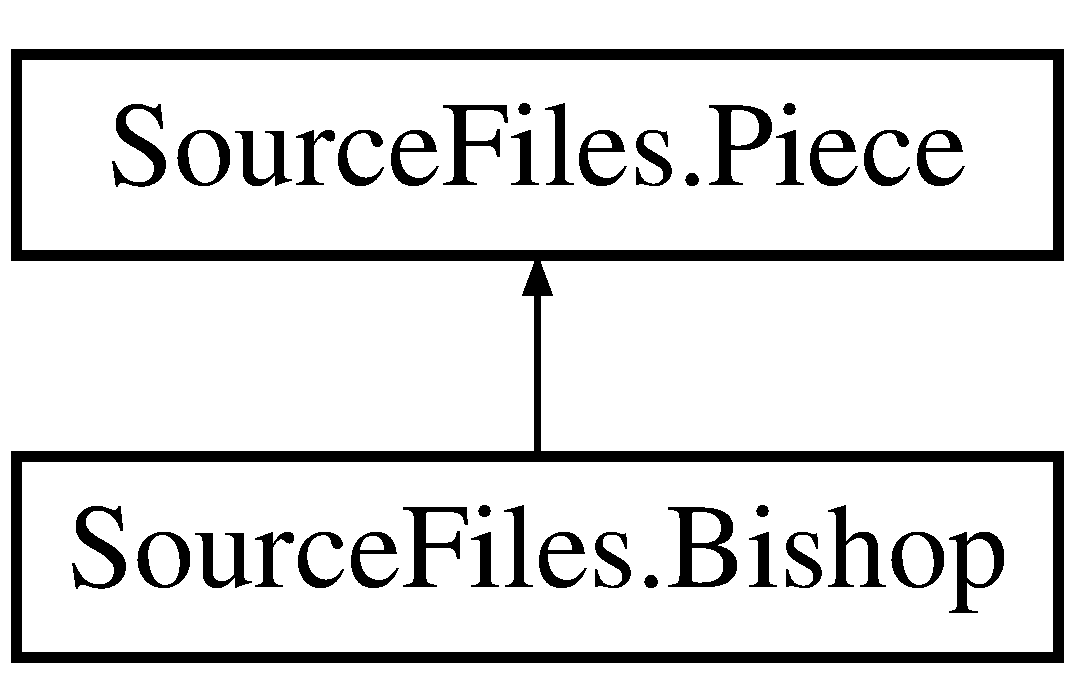
\includegraphics[height=2.000000cm]{class_source_files_1_1_bishop}
\end{center}
\end{figure}
\subsection*{Public Member Functions}
\begin{DoxyCompactItemize}
\item 
\mbox{\Hypertarget{class_source_files_1_1_bishop_a724b797ae52cff00d2de4d1313a350db}\label{class_source_files_1_1_bishop_a724b797ae52cff00d2de4d1313a350db}} 
{\bfseries Bishop} (int team)
\item 
\mbox{\Hypertarget{class_source_files_1_1_bishop_a6dab57f8f7853fb2f9761036b2fe6ada}\label{class_source_files_1_1_bishop_a6dab57f8f7853fb2f9761036b2fe6ada}} 
Array\+List$<$ \mbox{\hyperlink{class_source_files_1_1_coordinate}{Coordinate}} $>$ {\bfseries get\+Movement\+Path} (\mbox{\hyperlink{class_source_files_1_1_coordinate}{Coordinate}} start, \mbox{\hyperlink{class_source_files_1_1_coordinate}{Coordinate}} dest, \mbox{\hyperlink{class_source_files_1_1_field}{Field}} f)
\item 
\mbox{\Hypertarget{class_source_files_1_1_bishop_a468a6273cadc128e711bcb850860900e}\label{class_source_files_1_1_bishop_a468a6273cadc128e711bcb850860900e}} 
Array\+List$<$ \mbox{\hyperlink{class_source_files_1_1_coordinate}{Coordinate}} $>$ {\bfseries get\+All\+Possible\+Moves} (\mbox{\hyperlink{class_source_files_1_1_coordinate}{Coordinate}} start)
\item 
\mbox{\Hypertarget{class_source_files_1_1_bishop_abfc630755ddc003e009a699e66fadd8e}\label{class_source_files_1_1_bishop_abfc630755ddc003e009a699e66fadd8e}} 
Array\+List$<$ int\mbox{[}$\,$\mbox{]}$>$ {\bfseries draw\+Yourself} (int size)
\end{DoxyCompactItemize}
\subsection*{Additional Inherited Members}


The documentation for this class was generated from the following file\+:\begin{DoxyCompactItemize}
\item 
/\+Users/\+Charles\+B\+Swarts/eclipse-\/workspace/\+Chess\+Library/src/\+Source\+Files/Bishop.\+java\end{DoxyCompactItemize}

\hypertarget{class_tests_1_1_bishop_test}{}\section{Tests.\+Bishop\+Test Class Reference}
\label{class_tests_1_1_bishop_test}\index{Tests.\+Bishop\+Test@{Tests.\+Bishop\+Test}}
\subsection*{Public Member Functions}
\begin{DoxyCompactItemize}
\item 
\mbox{\Hypertarget{class_tests_1_1_bishop_test_ab00adb5639306021f32a58f6bc623f45}\label{class_tests_1_1_bishop_test_ab00adb5639306021f32a58f6bc623f45}} 
void {\bfseries cannot\+Move\+To\+Current\+Location\+Test} ()
\item 
\mbox{\Hypertarget{class_tests_1_1_bishop_test_a0684ff2350c3ab8a0e938f135a516453}\label{class_tests_1_1_bishop_test_a0684ff2350c3ab8a0e938f135a516453}} 
void {\bfseries move\+To\+Valid\+Locations\+Test} ()
\item 
\mbox{\Hypertarget{class_tests_1_1_bishop_test_ae926df81df4a15492ad7d92c2080f156}\label{class_tests_1_1_bishop_test_ae926df81df4a15492ad7d92c2080f156}} 
void {\bfseries move\+To\+Invalid\+Locations\+Test} ()
\item 
\mbox{\Hypertarget{class_tests_1_1_bishop_test_a6f92af0356f98f4a25e13b51562965a3}\label{class_tests_1_1_bishop_test_a6f92af0356f98f4a25e13b51562965a3}} 
void {\bfseries up\+To\+The\+Right\+Test} ()
\item 
\mbox{\Hypertarget{class_tests_1_1_bishop_test_a849ce7c7e62043925de4f38e085aecef}\label{class_tests_1_1_bishop_test_a849ce7c7e62043925de4f38e085aecef}} 
void {\bfseries down\+To\+The\+Right\+Test} ()
\item 
\mbox{\Hypertarget{class_tests_1_1_bishop_test_a345d82dd66b18a90abb348d3f5ee86d7}\label{class_tests_1_1_bishop_test_a345d82dd66b18a90abb348d3f5ee86d7}} 
void {\bfseries down\+To\+The\+Left\+Test} ()
\item 
\mbox{\Hypertarget{class_tests_1_1_bishop_test_a9807d86b86cf5a525aaac34e98c2c3e1}\label{class_tests_1_1_bishop_test_a9807d86b86cf5a525aaac34e98c2c3e1}} 
void {\bfseries up\+To\+The\+Left\+Test} ()
\end{DoxyCompactItemize}


The documentation for this class was generated from the following file\+:\begin{DoxyCompactItemize}
\item 
/\+Users/\+Charles\+B\+Swarts/eclipse-\/workspace/\+Chess\+Library/src/\+Tests/Bishop\+Test.\+java\end{DoxyCompactItemize}

\hypertarget{class_source_files_1_1_board}{}\section{Source\+Files.\+Board Class Reference}
\label{class_source_files_1_1_board}\index{Source\+Files.\+Board@{Source\+Files.\+Board}}
Inheritance diagram for Source\+Files.\+Board\+:\begin{figure}[H]
\begin{center}
\leavevmode
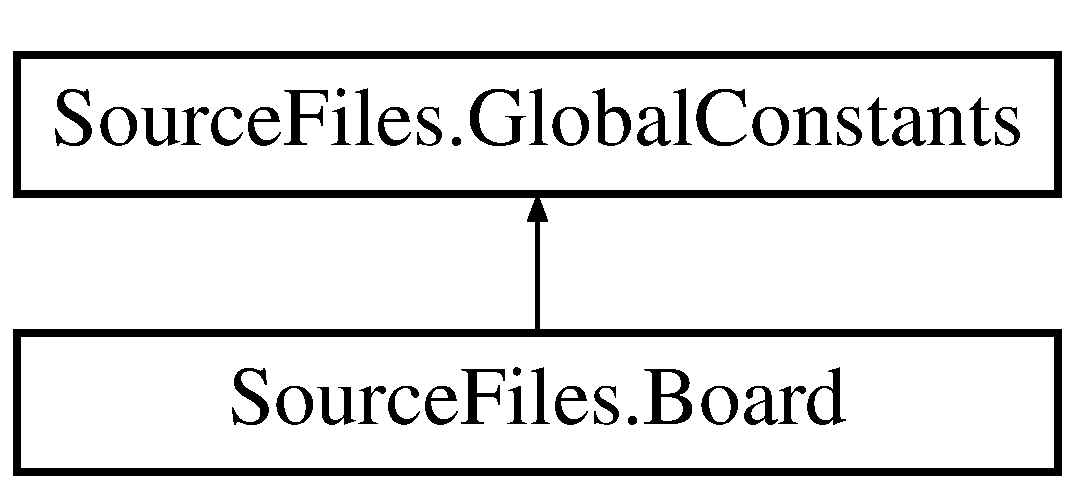
\includegraphics[height=2.000000cm]{class_source_files_1_1_board}
\end{center}
\end{figure}
\subsection*{Public Member Functions}
\begin{DoxyCompactItemize}
\item 
\mbox{\Hypertarget{class_source_files_1_1_board_a39388a321054ce264c99c559bbae91cf}\label{class_source_files_1_1_board_a39388a321054ce264c99c559bbae91cf}} 
{\bfseries Board} (int rows, int cols)
\item 
\mbox{\Hypertarget{class_source_files_1_1_board_abdd5495611adcce4a49deedf112d0c64}\label{class_source_files_1_1_board_abdd5495611adcce4a49deedf112d0c64}} 
int {\bfseries get\+Turn} ()
\item 
\mbox{\Hypertarget{class_source_files_1_1_board_a36176c6b86da18318e5f95614672ad3a}\label{class_source_files_1_1_board_a36176c6b86da18318e5f95614672ad3a}} 
\mbox{\hyperlink{class_source_files_1_1_field}{Field}} {\bfseries get\+Field} ()
\item 
\mbox{\Hypertarget{class_source_files_1_1_board_a953f1625ad648ec831b558fc830547eb}\label{class_source_files_1_1_board_a953f1625ad648ec831b558fc830547eb}} 
void {\bfseries add\+Piece} (\mbox{\hyperlink{class_source_files_1_1_piece}{Piece}} p, \mbox{\hyperlink{class_source_files_1_1_coordinate}{Coordinate}} c)
\item 
\mbox{\Hypertarget{class_source_files_1_1_board_a5101aefac80ed06f1eab3c1839a6c716}\label{class_source_files_1_1_board_a5101aefac80ed06f1eab3c1839a6c716}} 
int {\bfseries move} (\mbox{\hyperlink{class_source_files_1_1_coordinate}{Coordinate}} start, \mbox{\hyperlink{class_source_files_1_1_coordinate}{Coordinate}} dest)
\item 
\mbox{\Hypertarget{class_source_files_1_1_board_a01644b1564591a11e021a286b9ad7186}\label{class_source_files_1_1_board_a01644b1564591a11e021a286b9ad7186}} 
void {\bfseries undo\+Move} ()
\item 
\mbox{\Hypertarget{class_source_files_1_1_board_a14332f64be3e79eda891820ff888fc48}\label{class_source_files_1_1_board_a14332f64be3e79eda891820ff888fc48}} 
boolean {\bfseries in\+Check} (int team)
\item 
\mbox{\Hypertarget{class_source_files_1_1_board_a8e813074411332f3d9f523599680fbc9}\label{class_source_files_1_1_board_a8e813074411332f3d9f523599680fbc9}} 
boolean {\bfseries king\+Is\+Surrounded} (int team)
\item 
\mbox{\Hypertarget{class_source_files_1_1_board_a3e43e89aa25f6ce300fa910c745db7c8}\label{class_source_files_1_1_board_a3e43e89aa25f6ce300fa910c745db7c8}} 
boolean {\bfseries can\+Block\+To\+Escape\+Check} (int team)
\item 
\mbox{\Hypertarget{class_source_files_1_1_board_a015cf25758362c357cbe22c16d16ce8a}\label{class_source_files_1_1_board_a015cf25758362c357cbe22c16d16ce8a}} 
\mbox{\hyperlink{class_source_files_1_1_coordinate}{Coordinate}} {\bfseries find\+King} (int team)
\item 
\mbox{\Hypertarget{class_source_files_1_1_board_af2ecfd97a28c5bb54cd8e59c8e7669b3}\label{class_source_files_1_1_board_af2ecfd97a28c5bb54cd8e59c8e7669b3}} 
boolean {\bfseries is\+In\+Danger} (\mbox{\hyperlink{class_source_files_1_1_coordinate}{Coordinate}} dest)
\item 
\mbox{\Hypertarget{class_source_files_1_1_board_ad914cd023063965629caece5bb73e142}\label{class_source_files_1_1_board_ad914cd023063965629caece5bb73e142}} 
void {\bfseries setup\+Normal\+Game} ()
\end{DoxyCompactItemize}
\subsection*{Additional Inherited Members}


The documentation for this class was generated from the following file\+:\begin{DoxyCompactItemize}
\item 
/\+Users/\+Charles\+B\+Swarts/eclipse-\/workspace/\+Chess\+Library/src/\+Source\+Files/Board.\+java\end{DoxyCompactItemize}

\hypertarget{class_tests_1_1_board_test}{}\section{Tests.\+Board\+Test Class Reference}
\label{class_tests_1_1_board_test}\index{Tests.\+Board\+Test@{Tests.\+Board\+Test}}
\subsection*{Public Member Functions}
\begin{DoxyCompactItemize}
\item 
\mbox{\Hypertarget{class_tests_1_1_board_test_ab8064d4a263f1c5d09936f55d6d77dca}\label{class_tests_1_1_board_test_ab8064d4a263f1c5d09936f55d6d77dca}} 
void {\bfseries setup\+Chess\+Gametest} ()
\end{DoxyCompactItemize}


The documentation for this class was generated from the following file\+:\begin{DoxyCompactItemize}
\item 
/\+Users/\+Charles\+B\+Swarts/eclipse-\/workspace/\+Chess\+Library/src/\+Tests/Board\+Test.\+java\end{DoxyCompactItemize}

\hypertarget{class_g_u_i_1_1_colored_polygon}{}\section{G\+U\+I.\+Colored\+Polygon Class Reference}
\label{class_g_u_i_1_1_colored_polygon}\index{G\+U\+I.\+Colored\+Polygon@{G\+U\+I.\+Colored\+Polygon}}
Inheritance diagram for G\+U\+I.\+Colored\+Polygon\+:\begin{figure}[H]
\begin{center}
\leavevmode
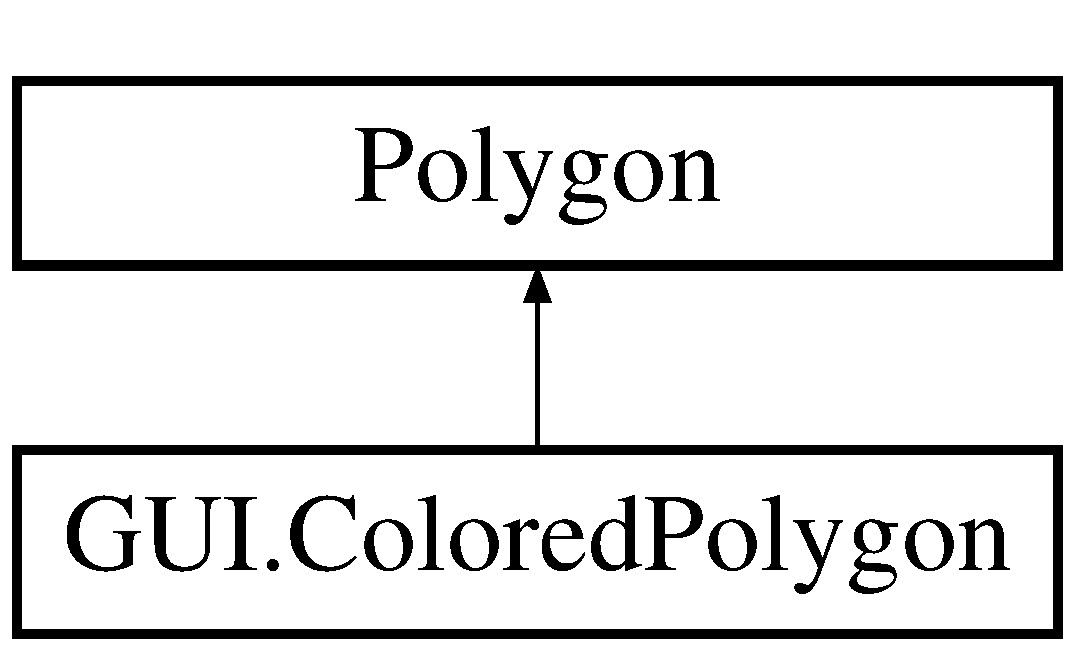
\includegraphics[height=2.000000cm]{class_g_u_i_1_1_colored_polygon}
\end{center}
\end{figure}
\subsection*{Public Member Functions}
\begin{DoxyCompactItemize}
\item 
\mbox{\Hypertarget{class_g_u_i_1_1_colored_polygon_ae79731531f6cc08cbbf0ca6e24856256}\label{class_g_u_i_1_1_colored_polygon_ae79731531f6cc08cbbf0ca6e24856256}} 
{\bfseries Colored\+Polygon} (int\mbox{[}$\,$\mbox{]} xpoints, int\mbox{[}$\,$\mbox{]} ypoints, int numpoints, int team)
\end{DoxyCompactItemize}
\subsection*{Public Attributes}
\begin{DoxyCompactItemize}
\item 
\mbox{\Hypertarget{class_g_u_i_1_1_colored_polygon_a6576e0c0d2970d3920b759aabf9f7a7d}\label{class_g_u_i_1_1_colored_polygon_a6576e0c0d2970d3920b759aabf9f7a7d}} 
int {\bfseries team}
\end{DoxyCompactItemize}


The documentation for this class was generated from the following file\+:\begin{DoxyCompactItemize}
\item 
/\+Users/\+Charles\+B\+Swarts/eclipse-\/workspace/\+Chess\+Library/src/\+G\+U\+I/Colored\+Polygon.\+java\end{DoxyCompactItemize}

\hypertarget{class_source_files_1_1_coordinate}{}\section{Source\+Files.\+Coordinate Class Reference}
\label{class_source_files_1_1_coordinate}\index{Source\+Files.\+Coordinate@{Source\+Files.\+Coordinate}}
\subsection*{Public Member Functions}
\begin{DoxyCompactItemize}
\item 
\mbox{\Hypertarget{class_source_files_1_1_coordinate_a42b6f0ed107bc33c60a95ca201ba674e}\label{class_source_files_1_1_coordinate_a42b6f0ed107bc33c60a95ca201ba674e}} 
{\bfseries Coordinate} (int i, int j)
\item 
\mbox{\Hypertarget{class_source_files_1_1_coordinate_aacd0c92f36535ff141a72ecb512c6ed7}\label{class_source_files_1_1_coordinate_aacd0c92f36535ff141a72ecb512c6ed7}} 
boolean {\bfseries eq} (\mbox{\hyperlink{class_source_files_1_1_coordinate}{Coordinate}} rhs)
\end{DoxyCompactItemize}
\subsection*{Public Attributes}
\begin{DoxyCompactItemize}
\item 
\mbox{\Hypertarget{class_source_files_1_1_coordinate_a439fe353b30f0dae43e6a26bcadd3381}\label{class_source_files_1_1_coordinate_a439fe353b30f0dae43e6a26bcadd3381}} 
int {\bfseries x}
\item 
\mbox{\Hypertarget{class_source_files_1_1_coordinate_a6ca661936240ac9143c61e8a8f6214ec}\label{class_source_files_1_1_coordinate_a6ca661936240ac9143c61e8a8f6214ec}} 
int {\bfseries y}
\end{DoxyCompactItemize}


The documentation for this class was generated from the following file\+:\begin{DoxyCompactItemize}
\item 
/\+Users/\+Charles\+B\+Swarts/eclipse-\/workspace/\+Chess\+Library/src/\+Source\+Files/Coordinate.\+java\end{DoxyCompactItemize}

\hypertarget{class_source_files_1_1_field}{}\section{Source\+Files.\+Field Class Reference}
\label{class_source_files_1_1_field}\index{Source\+Files.\+Field@{Source\+Files.\+Field}}
\subsection*{Public Member Functions}
\begin{DoxyCompactItemize}
\item 
\mbox{\Hypertarget{class_source_files_1_1_field_a51a2df71be8b7c3aa45982648794b60d}\label{class_source_files_1_1_field_a51a2df71be8b7c3aa45982648794b60d}} 
{\bfseries Field} (int rows, int cols)
\item 
\mbox{\Hypertarget{class_source_files_1_1_field_a39605884440965bdd30128b68a6bbea3}\label{class_source_files_1_1_field_a39605884440965bdd30128b68a6bbea3}} 
\mbox{\hyperlink{class_source_files_1_1_piece}{Piece}} {\bfseries at} (\mbox{\hyperlink{class_source_files_1_1_coordinate}{Coordinate}} c)
\item 
\mbox{\Hypertarget{class_source_files_1_1_field_a0c37dd4602bf2c74364294469e20e286}\label{class_source_files_1_1_field_a0c37dd4602bf2c74364294469e20e286}} 
void {\bfseries set} (\mbox{\hyperlink{class_source_files_1_1_coordinate}{Coordinate}} c, \mbox{\hyperlink{class_source_files_1_1_piece}{Piece}} p)
\item 
\mbox{\Hypertarget{class_source_files_1_1_field_a67894dae4f9cdc813cc31abadbe1c813}\label{class_source_files_1_1_field_a67894dae4f9cdc813cc31abadbe1c813}} 
boolean {\bfseries in\+Bounds} (\mbox{\hyperlink{class_source_files_1_1_coordinate}{Coordinate}} c)
\item 
\mbox{\Hypertarget{class_source_files_1_1_field_a5a7c1a071941e7fa0361121ad7a3ec9a}\label{class_source_files_1_1_field_a5a7c1a071941e7fa0361121ad7a3ec9a}} 
Array\+List$<$ \mbox{\hyperlink{class_source_files_1_1_coordinate}{Coordinate}} $>$ {\bfseries no\+Nulls\+Traverse} ()
\end{DoxyCompactItemize}


The documentation for this class was generated from the following file\+:\begin{DoxyCompactItemize}
\item 
/\+Users/\+Charles\+B\+Swarts/eclipse-\/workspace/\+Chess\+Library/src/\+Source\+Files/Field.\+java\end{DoxyCompactItemize}

\hypertarget{class_source_files_1_1_global_constants}{}\section{Source\+Files.\+Global\+Constants Class Reference}
\label{class_source_files_1_1_global_constants}\index{Source\+Files.\+Global\+Constants@{Source\+Files.\+Global\+Constants}}
Inheritance diagram for Source\+Files.\+Global\+Constants\+:\begin{figure}[H]
\begin{center}
\leavevmode
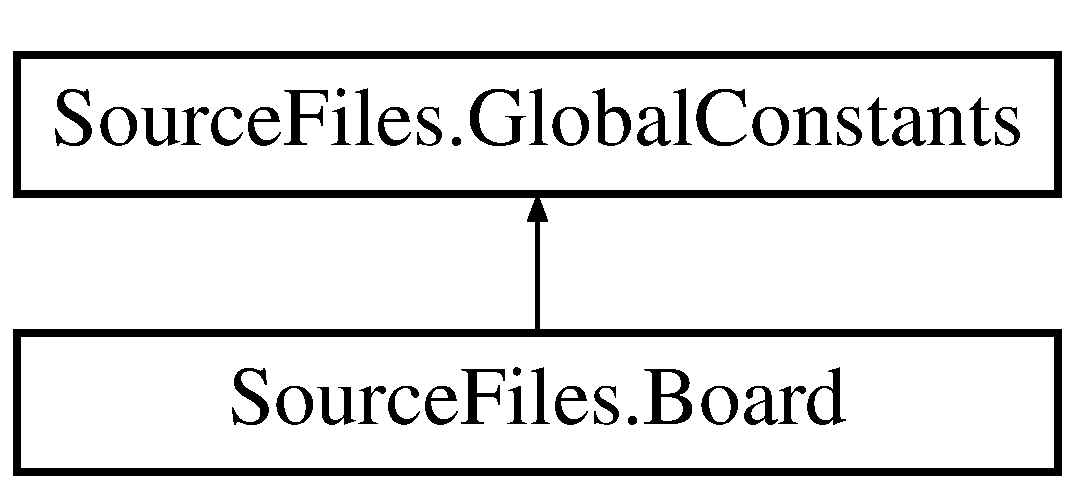
\includegraphics[height=2.000000cm]{class_source_files_1_1_global_constants}
\end{center}
\end{figure}
\subsection*{Static Protected Attributes}
\begin{DoxyCompactItemize}
\item 
\mbox{\Hypertarget{class_source_files_1_1_global_constants_a6847ad2c5cdc53aada086e53f4b91199}\label{class_source_files_1_1_global_constants_a6847ad2c5cdc53aada086e53f4b91199}} 
static final int {\bfseries N\+O\+M\+I\+N\+AL} = 0
\item 
\mbox{\Hypertarget{class_source_files_1_1_global_constants_a25997c80ffd128c057610ac9d8665857}\label{class_source_files_1_1_global_constants_a25997c80ffd128c057610ac9d8665857}} 
static final int {\bfseries N\+O\+T\+H\+I\+NG} = 0
\item 
\mbox{\Hypertarget{class_source_files_1_1_global_constants_a5675b48c6bcd43cae87cc035a6cf8d15}\label{class_source_files_1_1_global_constants_a5675b48c6bcd43cae87cc035a6cf8d15}} 
static final int {\bfseries K\+I\+NG} = 1
\item 
\mbox{\Hypertarget{class_source_files_1_1_global_constants_a61afcbc1e8a6747ece66d1f9583e43f2}\label{class_source_files_1_1_global_constants_a61afcbc1e8a6747ece66d1f9583e43f2}} 
static final int {\bfseries Q\+U\+E\+EN} = 2
\item 
\mbox{\Hypertarget{class_source_files_1_1_global_constants_a3423c8805d09c4cdf737ab9d8834bb33}\label{class_source_files_1_1_global_constants_a3423c8805d09c4cdf737ab9d8834bb33}} 
static final int {\bfseries R\+O\+OK} = 3
\item 
\mbox{\Hypertarget{class_source_files_1_1_global_constants_a9f1e20b75cc3a16f485f07fac3560ab2}\label{class_source_files_1_1_global_constants_a9f1e20b75cc3a16f485f07fac3560ab2}} 
static final int {\bfseries B\+I\+S\+H\+OP} = 4
\item 
\mbox{\Hypertarget{class_source_files_1_1_global_constants_a32be8b8f114b1422a9ab4b776b7c4681}\label{class_source_files_1_1_global_constants_a32be8b8f114b1422a9ab4b776b7c4681}} 
static final int {\bfseries K\+N\+I\+G\+HT} = 5
\item 
\mbox{\Hypertarget{class_source_files_1_1_global_constants_a79bb47e69f65ddcbd19fc451daa17de0}\label{class_source_files_1_1_global_constants_a79bb47e69f65ddcbd19fc451daa17de0}} 
static final int {\bfseries P\+A\+WN} = 6
\item 
\mbox{\Hypertarget{class_source_files_1_1_global_constants_a8e628635720c0648896506421cb6f426}\label{class_source_files_1_1_global_constants_a8e628635720c0648896506421cb6f426}} 
static final int {\bfseries M\+U\+S\+T\+\_\+\+M\+O\+V\+E\+\_\+\+A\+\_\+\+P\+I\+E\+CE} = 7
\item 
\mbox{\Hypertarget{class_source_files_1_1_global_constants_a9ef9278453eb61547d5986c056eb77d2}\label{class_source_files_1_1_global_constants_a9ef9278453eb61547d5986c056eb77d2}} 
static final int {\bfseries O\+U\+T\+\_\+\+O\+F\+\_\+\+T\+U\+RN} = 8
\item 
\mbox{\Hypertarget{class_source_files_1_1_global_constants_aac542b6414d8eac71faaf819bfa2280d}\label{class_source_files_1_1_global_constants_aac542b6414d8eac71faaf819bfa2280d}} 
static final int {\bfseries C\+A\+N\+N\+O\+T\+\_\+\+A\+T\+T\+A\+C\+K\+\_\+\+Y\+O\+U\+R\+\_\+\+O\+W\+N\+\_\+\+P\+I\+E\+CE} = 9
\item 
\mbox{\Hypertarget{class_source_files_1_1_global_constants_a61c6486b826536ce41427a11dbeb1d1d}\label{class_source_files_1_1_global_constants_a61c6486b826536ce41427a11dbeb1d1d}} 
static final int {\bfseries A\+T\+T\+A\+C\+K\+\_\+\+P\+A\+T\+H\+\_\+\+I\+S\+\_\+\+N\+O\+T\+\_\+\+C\+L\+E\+AR} = 10
\item 
\mbox{\Hypertarget{class_source_files_1_1_global_constants_a45eb62b489a8eb28e2b80ef91059d15c}\label{class_source_files_1_1_global_constants_a45eb62b489a8eb28e2b80ef91059d15c}} 
static final int {\bfseries M\+O\+V\+E\+\_\+\+I\+S\+\_\+\+N\+O\+T\+\_\+\+P\+O\+S\+S\+I\+B\+LE} = 15
\item 
\mbox{\Hypertarget{class_source_files_1_1_global_constants_adacc7da311b47ca668e788ac55dff028}\label{class_source_files_1_1_global_constants_adacc7da311b47ca668e788ac55dff028}} 
static final int {\bfseries C\+H\+E\+CK} = 11
\item 
\mbox{\Hypertarget{class_source_files_1_1_global_constants_ae772ac01db3f38b565b54721b0070220}\label{class_source_files_1_1_global_constants_ae772ac01db3f38b565b54721b0070220}} 
static final int {\bfseries C\+H\+E\+C\+K\+M\+A\+TE} = 12
\item 
\mbox{\Hypertarget{class_source_files_1_1_global_constants_a49cd457881034d16fd1c6312447a6a90}\label{class_source_files_1_1_global_constants_a49cd457881034d16fd1c6312447a6a90}} 
static final int {\bfseries S\+T\+A\+L\+E\+M\+A\+TE} = 13
\item 
\mbox{\Hypertarget{class_source_files_1_1_global_constants_a9ea2080c41421e9bf741935a5b8660b3}\label{class_source_files_1_1_global_constants_a9ea2080c41421e9bf741935a5b8660b3}} 
static final int {\bfseries M\+U\+S\+T\+\_\+\+E\+S\+C\+A\+P\+E\+\_\+\+C\+H\+E\+CK} = 14
\end{DoxyCompactItemize}


The documentation for this class was generated from the following file\+:\begin{DoxyCompactItemize}
\item 
/\+Users/\+Charles\+B\+Swarts/eclipse-\/workspace/\+Chess\+Library/src/\+Source\+Files/Global\+Constants.\+java\end{DoxyCompactItemize}

\hypertarget{class_g_u_i_1_1_g_u_i_main}{}\section{G\+U\+I.\+G\+U\+I\+Main Class Reference}
\label{class_g_u_i_1_1_g_u_i_main}\index{G\+U\+I.\+G\+U\+I\+Main@{G\+U\+I.\+G\+U\+I\+Main}}
Inheritance diagram for G\+U\+I.\+G\+U\+I\+Main\+:\begin{figure}[H]
\begin{center}
\leavevmode
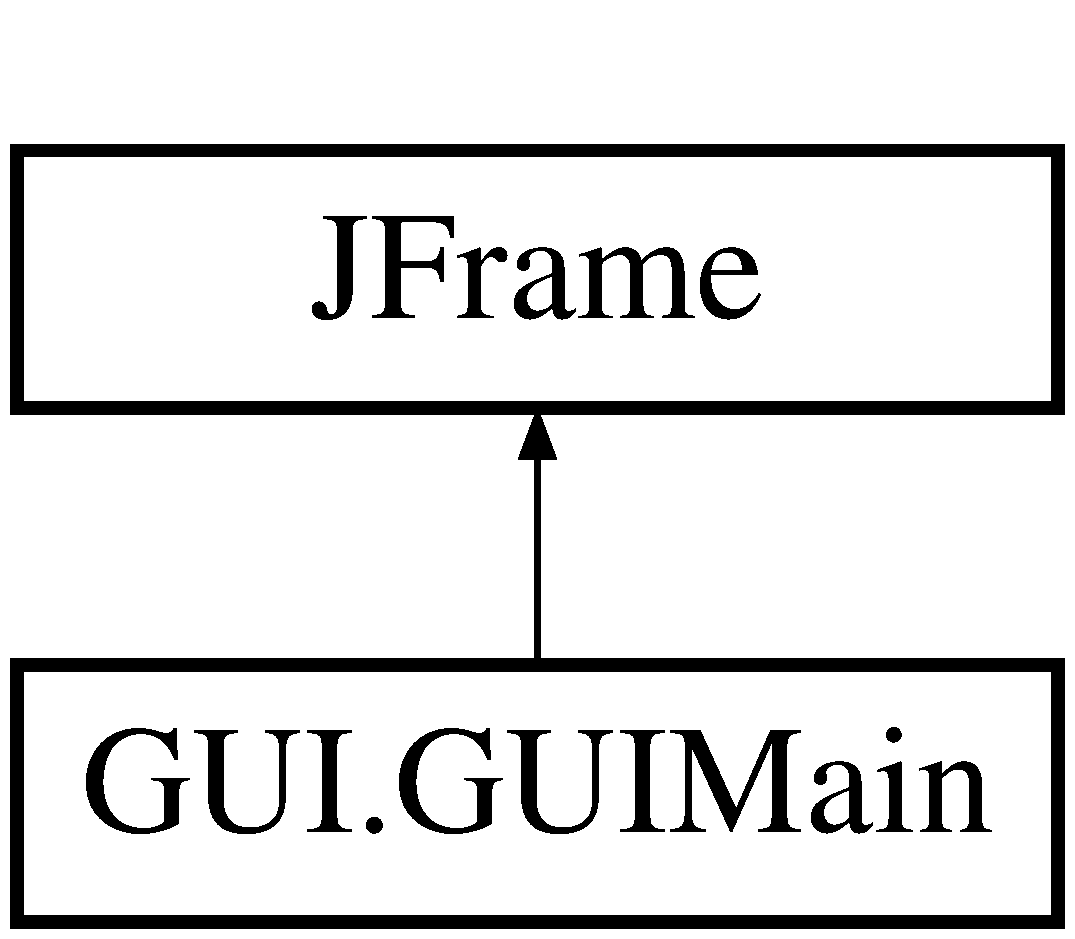
\includegraphics[height=2.000000cm]{class_g_u_i_1_1_g_u_i_main}
\end{center}
\end{figure}
\subsection*{Static Public Member Functions}
\begin{DoxyCompactItemize}
\item 
\mbox{\Hypertarget{class_g_u_i_1_1_g_u_i_main_aa7064fd358c4134460d9974c363674b5}\label{class_g_u_i_1_1_g_u_i_main_aa7064fd358c4134460d9974c363674b5}} 
static void {\bfseries main} (String\mbox{[}$\,$\mbox{]} args)
\end{DoxyCompactItemize}


The documentation for this class was generated from the following file\+:\begin{DoxyCompactItemize}
\item 
/\+Users/\+Charles\+B\+Swarts/eclipse-\/workspace/\+Chess\+Library/src/\+G\+U\+I/G\+U\+I\+Main.\+java\end{DoxyCompactItemize}

\hypertarget{class_source_files_1_1_king}{}\section{Source\+Files.\+King Class Reference}
\label{class_source_files_1_1_king}\index{Source\+Files.\+King@{Source\+Files.\+King}}
Inheritance diagram for Source\+Files.\+King\+:\begin{figure}[H]
\begin{center}
\leavevmode
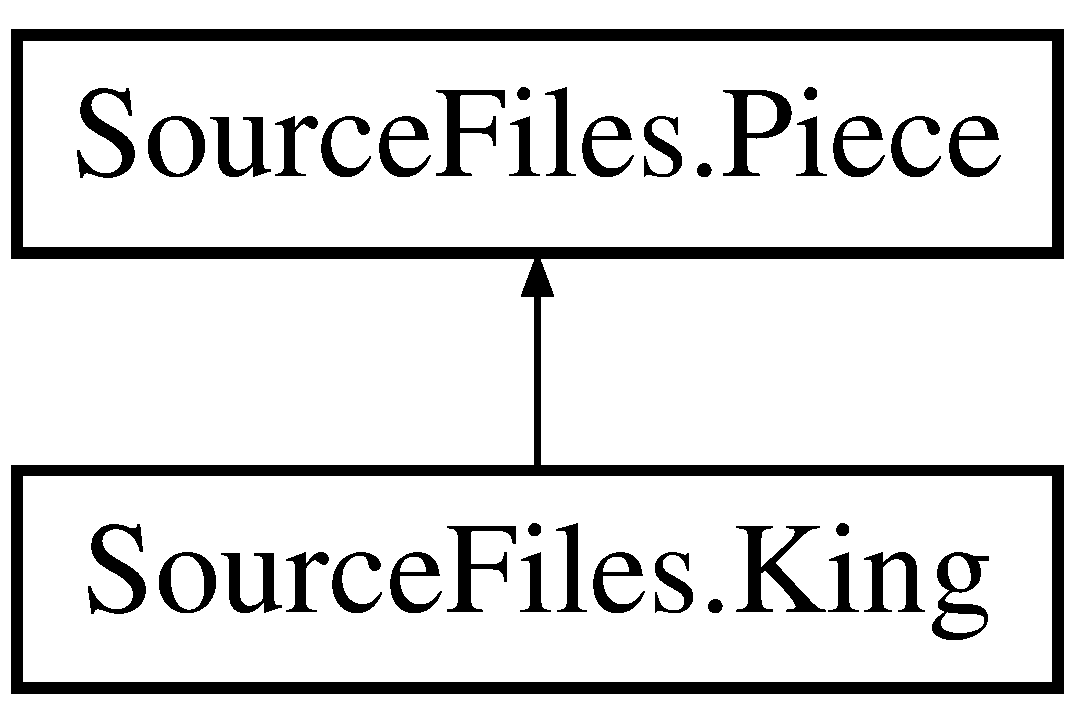
\includegraphics[height=2.000000cm]{class_source_files_1_1_king}
\end{center}
\end{figure}
\subsection*{Public Member Functions}
\begin{DoxyCompactItemize}
\item 
\mbox{\Hypertarget{class_source_files_1_1_king_a9450f56d32e3b20edd87b76344cd086d}\label{class_source_files_1_1_king_a9450f56d32e3b20edd87b76344cd086d}} 
{\bfseries King} (int team)
\item 
\mbox{\Hypertarget{class_source_files_1_1_king_a55d2cf7f6205db10e7d221b1cdf27bfb}\label{class_source_files_1_1_king_a55d2cf7f6205db10e7d221b1cdf27bfb}} 
Array\+List$<$ \mbox{\hyperlink{class_source_files_1_1_coordinate}{Coordinate}} $>$ {\bfseries get\+Movement\+Path} (\mbox{\hyperlink{class_source_files_1_1_coordinate}{Coordinate}} start, \mbox{\hyperlink{class_source_files_1_1_coordinate}{Coordinate}} dest, \mbox{\hyperlink{class_source_files_1_1_field}{Field}} f)
\item 
\mbox{\Hypertarget{class_source_files_1_1_king_ad48c205a3719de5d9a4637ae3b779df7}\label{class_source_files_1_1_king_ad48c205a3719de5d9a4637ae3b779df7}} 
Array\+List$<$ \mbox{\hyperlink{class_source_files_1_1_coordinate}{Coordinate}} $>$ {\bfseries get\+All\+Possible\+Moves} (\mbox{\hyperlink{class_source_files_1_1_coordinate}{Coordinate}} c)
\item 
\mbox{\Hypertarget{class_source_files_1_1_king_ac8459ed5a52a831e563b4d5b36d75716}\label{class_source_files_1_1_king_ac8459ed5a52a831e563b4d5b36d75716}} 
Array\+List$<$ int\mbox{[}$\,$\mbox{]}$>$ {\bfseries draw\+Yourself} (int size)
\end{DoxyCompactItemize}
\subsection*{Additional Inherited Members}


The documentation for this class was generated from the following file\+:\begin{DoxyCompactItemize}
\item 
/\+Users/\+Charles\+B\+Swarts/eclipse-\/workspace/\+Chess\+Library/src/\+Source\+Files/King.\+java\end{DoxyCompactItemize}

\hypertarget{class_tests_1_1_king_test}{}\section{Tests.\+King\+Test Class Reference}
\label{class_tests_1_1_king_test}\index{Tests.\+King\+Test@{Tests.\+King\+Test}}
\subsection*{Public Member Functions}
\begin{DoxyCompactItemize}
\item 
\mbox{\Hypertarget{class_tests_1_1_king_test_aef386a444d2f1c46dd4559e303633a16}\label{class_tests_1_1_king_test_aef386a444d2f1c46dd4559e303633a16}} 
void {\bfseries one\+Test\+To\+Rule\+Them\+All} ()
\end{DoxyCompactItemize}


The documentation for this class was generated from the following file\+:\begin{DoxyCompactItemize}
\item 
/\+Users/\+Charles\+B\+Swarts/eclipse-\/workspace/\+Chess\+Library/src/\+Tests/King\+Test.\+java\end{DoxyCompactItemize}

\hypertarget{class_source_files_1_1_knight}{}\section{Source\+Files.\+Knight Class Reference}
\label{class_source_files_1_1_knight}\index{Source\+Files.\+Knight@{Source\+Files.\+Knight}}
Inheritance diagram for Source\+Files.\+Knight\+:\begin{figure}[H]
\begin{center}
\leavevmode
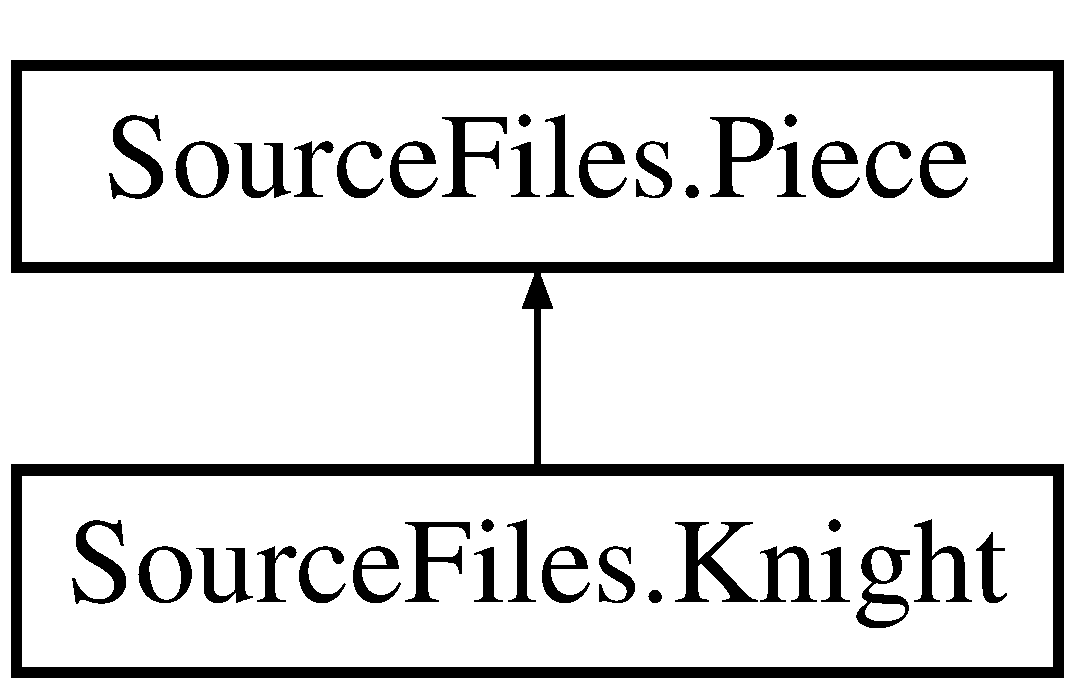
\includegraphics[height=2.000000cm]{class_source_files_1_1_knight}
\end{center}
\end{figure}
\subsection*{Public Member Functions}
\begin{DoxyCompactItemize}
\item 
\mbox{\Hypertarget{class_source_files_1_1_knight_a6cee1a1244b4e5375f9c45a9f1ad5ea3}\label{class_source_files_1_1_knight_a6cee1a1244b4e5375f9c45a9f1ad5ea3}} 
{\bfseries Knight} (int team)
\item 
\mbox{\Hypertarget{class_source_files_1_1_knight_a4d4e8c303d344065929ae708f08a7872}\label{class_source_files_1_1_knight_a4d4e8c303d344065929ae708f08a7872}} 
Array\+List$<$ \mbox{\hyperlink{class_source_files_1_1_coordinate}{Coordinate}} $>$ {\bfseries get\+Movement\+Path} (\mbox{\hyperlink{class_source_files_1_1_coordinate}{Coordinate}} start, \mbox{\hyperlink{class_source_files_1_1_coordinate}{Coordinate}} dest, \mbox{\hyperlink{class_source_files_1_1_field}{Field}} f)
\item 
\mbox{\Hypertarget{class_source_files_1_1_knight_a6cf1a8dfefede13ab9c1fb37ceebf79b}\label{class_source_files_1_1_knight_a6cf1a8dfefede13ab9c1fb37ceebf79b}} 
Array\+List$<$ \mbox{\hyperlink{class_source_files_1_1_coordinate}{Coordinate}} $>$ {\bfseries get\+All\+Possible\+Moves} (\mbox{\hyperlink{class_source_files_1_1_coordinate}{Coordinate}} start)
\item 
\mbox{\Hypertarget{class_source_files_1_1_knight_a82830375663170285bf38b9273a8571f}\label{class_source_files_1_1_knight_a82830375663170285bf38b9273a8571f}} 
Array\+List$<$ int\mbox{[}$\,$\mbox{]}$>$ {\bfseries draw\+Yourself} (int size)
\end{DoxyCompactItemize}
\subsection*{Additional Inherited Members}


The documentation for this class was generated from the following file\+:\begin{DoxyCompactItemize}
\item 
/\+Users/\+Charles\+B\+Swarts/eclipse-\/workspace/\+Chess\+Library/src/\+Source\+Files/Knight.\+java\end{DoxyCompactItemize}

\hypertarget{class_tests_1_1_knight_tests}{}\section{Tests.\+Knight\+Tests Class Reference}
\label{class_tests_1_1_knight_tests}\index{Tests.\+Knight\+Tests@{Tests.\+Knight\+Tests}}
\subsection*{Public Member Functions}
\begin{DoxyCompactItemize}
\item 
\mbox{\Hypertarget{class_tests_1_1_knight_tests_afdbd552cb2923f8c8713acb7aed18988}\label{class_tests_1_1_knight_tests_afdbd552cb2923f8c8713acb7aed18988}} 
void {\bfseries correct\+Knight\+Moves} ()
\item 
\mbox{\Hypertarget{class_tests_1_1_knight_tests_a36198195b7c415dfd173cd75b463268f}\label{class_tests_1_1_knight_tests_a36198195b7c415dfd173cd75b463268f}} 
void {\bfseries move\+To\+Invalid\+Locations\+Test} ()
\end{DoxyCompactItemize}


The documentation for this class was generated from the following file\+:\begin{DoxyCompactItemize}
\item 
/\+Users/\+Charles\+B\+Swarts/eclipse-\/workspace/\+Chess\+Library/src/\+Tests/Knight\+Tests.\+java\end{DoxyCompactItemize}

\hypertarget{class_source_files_1_1_move_record}{}\section{Source\+Files.\+Move\+Record Class Reference}
\label{class_source_files_1_1_move_record}\index{Source\+Files.\+Move\+Record@{Source\+Files.\+Move\+Record}}
\subsection*{Public Member Functions}
\begin{DoxyCompactItemize}
\item 
\mbox{\Hypertarget{class_source_files_1_1_move_record_a6ea76c8157cf0071099c13b779d153a3}\label{class_source_files_1_1_move_record_a6ea76c8157cf0071099c13b779d153a3}} 
{\bfseries Move\+Record} (\mbox{\hyperlink{class_source_files_1_1_coordinate}{Coordinate}} start, \mbox{\hyperlink{class_source_files_1_1_coordinate}{Coordinate}} dest, \mbox{\hyperlink{class_source_files_1_1_piece}{Piece}} attacker, \mbox{\hyperlink{class_source_files_1_1_piece}{Piece}} target)
\end{DoxyCompactItemize}
\subsection*{Public Attributes}
\begin{DoxyCompactItemize}
\item 
\mbox{\Hypertarget{class_source_files_1_1_move_record_ac7071333089312aa1034c69cde5310bb}\label{class_source_files_1_1_move_record_ac7071333089312aa1034c69cde5310bb}} 
\mbox{\hyperlink{class_source_files_1_1_coordinate}{Coordinate}} {\bfseries start}
\item 
\mbox{\Hypertarget{class_source_files_1_1_move_record_a3b78c14d9053b0c8dc65d06503da3767}\label{class_source_files_1_1_move_record_a3b78c14d9053b0c8dc65d06503da3767}} 
\mbox{\hyperlink{class_source_files_1_1_coordinate}{Coordinate}} {\bfseries dest}
\item 
\mbox{\Hypertarget{class_source_files_1_1_move_record_a969b8ed3bcaa2524fb2a9458d6771b24}\label{class_source_files_1_1_move_record_a969b8ed3bcaa2524fb2a9458d6771b24}} 
\mbox{\hyperlink{class_source_files_1_1_piece}{Piece}} {\bfseries attacker}
\item 
\mbox{\Hypertarget{class_source_files_1_1_move_record_af390bf9e25008e5d301fa0ddf04a37ed}\label{class_source_files_1_1_move_record_af390bf9e25008e5d301fa0ddf04a37ed}} 
\mbox{\hyperlink{class_source_files_1_1_piece}{Piece}} {\bfseries target}
\end{DoxyCompactItemize}


The documentation for this class was generated from the following file\+:\begin{DoxyCompactItemize}
\item 
/\+Users/\+Charles\+B\+Swarts/eclipse-\/workspace/\+Chess\+Library/src/\+Source\+Files/Move\+Record.\+java\end{DoxyCompactItemize}

\hypertarget{class_source_files_1_1_pawn}{}\section{Source\+Files.\+Pawn Class Reference}
\label{class_source_files_1_1_pawn}\index{Source\+Files.\+Pawn@{Source\+Files.\+Pawn}}
Inheritance diagram for Source\+Files.\+Pawn\+:\begin{figure}[H]
\begin{center}
\leavevmode
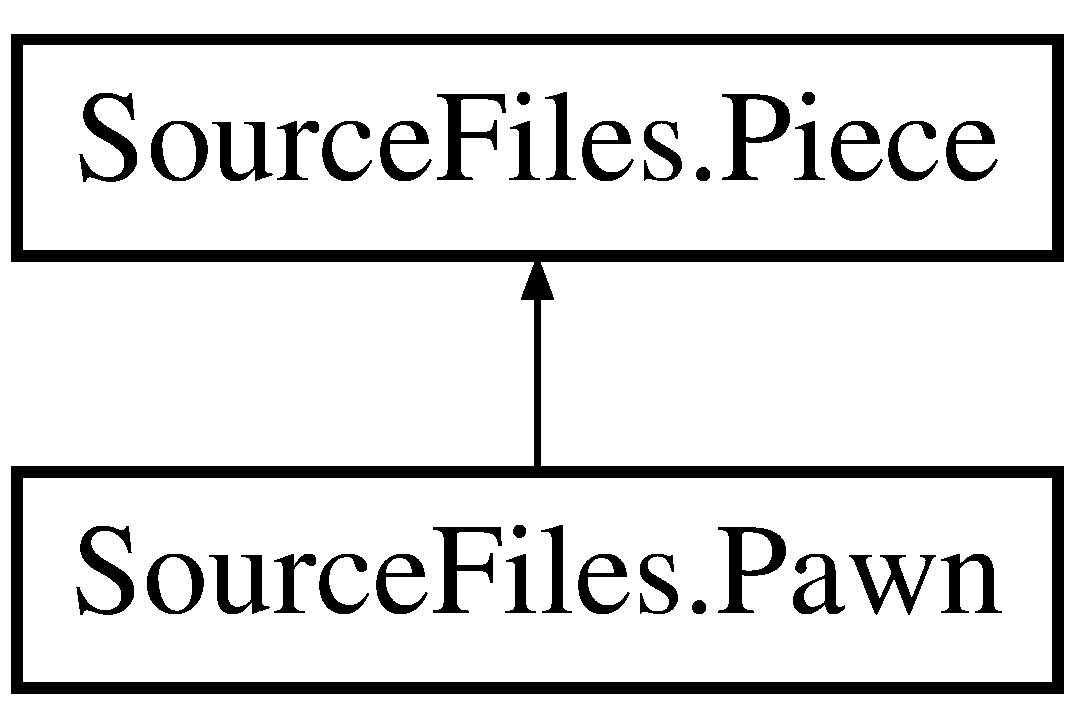
\includegraphics[height=2.000000cm]{class_source_files_1_1_pawn}
\end{center}
\end{figure}
\subsection*{Public Member Functions}
\begin{DoxyCompactItemize}
\item 
\mbox{\Hypertarget{class_source_files_1_1_pawn_ac2fee5b5a4ecfe6863eab93c4222e1ad}\label{class_source_files_1_1_pawn_ac2fee5b5a4ecfe6863eab93c4222e1ad}} 
{\bfseries Pawn} (int team)
\item 
\mbox{\Hypertarget{class_source_files_1_1_pawn_a7f49a265bc09fe040dab5328d1ffa41e}\label{class_source_files_1_1_pawn_a7f49a265bc09fe040dab5328d1ffa41e}} 
Array\+List$<$ \mbox{\hyperlink{class_source_files_1_1_coordinate}{Coordinate}} $>$ {\bfseries get\+Movement\+Path} (\mbox{\hyperlink{class_source_files_1_1_coordinate}{Coordinate}} start, \mbox{\hyperlink{class_source_files_1_1_coordinate}{Coordinate}} dest, \mbox{\hyperlink{class_source_files_1_1_field}{Field}} field)
\item 
\mbox{\Hypertarget{class_source_files_1_1_pawn_aa7318cf3aaeefdf1fe5f508dbd0d1e56}\label{class_source_files_1_1_pawn_aa7318cf3aaeefdf1fe5f508dbd0d1e56}} 
Array\+List$<$ \mbox{\hyperlink{class_source_files_1_1_coordinate}{Coordinate}} $>$ {\bfseries get\+All\+Possible\+Moves} (\mbox{\hyperlink{class_source_files_1_1_coordinate}{Coordinate}} start)
\item 
\mbox{\Hypertarget{class_source_files_1_1_pawn_ae78004729d2966d6b2f827ab200c4415}\label{class_source_files_1_1_pawn_ae78004729d2966d6b2f827ab200c4415}} 
Array\+List$<$ int\mbox{[}$\,$\mbox{]}$>$ {\bfseries draw\+Yourself} (int size)
\end{DoxyCompactItemize}
\subsection*{Additional Inherited Members}


The documentation for this class was generated from the following file\+:\begin{DoxyCompactItemize}
\item 
/\+Users/\+Charles\+B\+Swarts/eclipse-\/workspace/\+Chess\+Library/src/\+Source\+Files/Pawn.\+java\end{DoxyCompactItemize}

\hypertarget{class_tests_1_1_pawn_tests}{}\section{Tests.\+Pawn\+Tests Class Reference}
\label{class_tests_1_1_pawn_tests}\index{Tests.\+Pawn\+Tests@{Tests.\+Pawn\+Tests}}
\subsection*{Public Member Functions}
\begin{DoxyCompactItemize}
\item 
\mbox{\Hypertarget{class_tests_1_1_pawn_tests_a38e429241dcc2ad5ccfdee2b4d1b86e8}\label{class_tests_1_1_pawn_tests_a38e429241dcc2ad5ccfdee2b4d1b86e8}} 
void {\bfseries move1\+Test} ()
\item 
\mbox{\Hypertarget{class_tests_1_1_pawn_tests_a471cf3effb997ffac9c70d24780bc94b}\label{class_tests_1_1_pawn_tests_a471cf3effb997ffac9c70d24780bc94b}} 
void {\bfseries move2\+Test} ()
\item 
\mbox{\Hypertarget{class_tests_1_1_pawn_tests_a178ebd0459ba6a58c2a6dd8c34394d66}\label{class_tests_1_1_pawn_tests_a178ebd0459ba6a58c2a6dd8c34394d66}} 
void {\bfseries move\+Two\+In\+Subsequent\+Test} ()
\item 
\mbox{\Hypertarget{class_tests_1_1_pawn_tests_aa57ba1a300c2ae88e8abf71e24d89eae}\label{class_tests_1_1_pawn_tests_aa57ba1a300c2ae88e8abf71e24d89eae}} 
void {\bfseries diagonal\+Attack\+Test} ()
\item 
\mbox{\Hypertarget{class_tests_1_1_pawn_tests_aad3574dfffe7eb3771f68404801045ee}\label{class_tests_1_1_pawn_tests_aad3574dfffe7eb3771f68404801045ee}} 
void {\bfseries move\+Backwards\+And\+Sideways\+Test} ()
\end{DoxyCompactItemize}


The documentation for this class was generated from the following file\+:\begin{DoxyCompactItemize}
\item 
/\+Users/\+Charles\+B\+Swarts/eclipse-\/workspace/\+Chess\+Library/src/\+Tests/Pawn\+Tests.\+java\end{DoxyCompactItemize}

\hypertarget{class_source_files_1_1_piece}{}\section{Source\+Files.\+Piece Class Reference}
\label{class_source_files_1_1_piece}\index{Source\+Files.\+Piece@{Source\+Files.\+Piece}}
Inheritance diagram for Source\+Files.\+Piece\+:\begin{figure}[H]
\begin{center}
\leavevmode
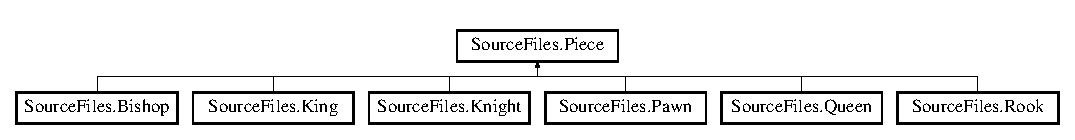
\includegraphics[height=1.435897cm]{class_source_files_1_1_piece}
\end{center}
\end{figure}
\subsection*{Public Member Functions}
\begin{DoxyCompactItemize}
\item 
\mbox{\Hypertarget{class_source_files_1_1_piece_a9202b7ac4e29e14713178189ede3e3bb}\label{class_source_files_1_1_piece_a9202b7ac4e29e14713178189ede3e3bb}} 
abstract Array\+List$<$ \mbox{\hyperlink{class_source_files_1_1_coordinate}{Coordinate}} $>$ {\bfseries get\+Movement\+Path} (\mbox{\hyperlink{class_source_files_1_1_coordinate}{Coordinate}} start, \mbox{\hyperlink{class_source_files_1_1_coordinate}{Coordinate}} dest, \mbox{\hyperlink{class_source_files_1_1_field}{Field}} f)
\item 
\mbox{\Hypertarget{class_source_files_1_1_piece_a3d4023342377075e32823252d4177813}\label{class_source_files_1_1_piece_a3d4023342377075e32823252d4177813}} 
abstract Array\+List$<$ \mbox{\hyperlink{class_source_files_1_1_coordinate}{Coordinate}} $>$ {\bfseries get\+All\+Possible\+Moves} (\mbox{\hyperlink{class_source_files_1_1_coordinate}{Coordinate}} start)
\item 
\mbox{\Hypertarget{class_source_files_1_1_piece_a2b70c2f3bff883dca506fb3380c1e0b0}\label{class_source_files_1_1_piece_a2b70c2f3bff883dca506fb3380c1e0b0}} 
\mbox{\hyperlink{class_g_u_i_1_1_colored_polygon}{Colored\+Polygon}} {\bfseries get\+Colored\+Polygon} (int size)
\item 
\mbox{\Hypertarget{class_source_files_1_1_piece_ad78c3c615a21583d0c3864676a7effe1}\label{class_source_files_1_1_piece_ad78c3c615a21583d0c3864676a7effe1}} 
boolean {\bfseries can\+Move} (\mbox{\hyperlink{class_source_files_1_1_coordinate}{Coordinate}} start, \mbox{\hyperlink{class_source_files_1_1_coordinate}{Coordinate}} dest, \mbox{\hyperlink{class_source_files_1_1_field}{Field}} field)
\item 
\mbox{\Hypertarget{class_source_files_1_1_piece_af32e028a8380a2510f53640fdd21f8e1}\label{class_source_files_1_1_piece_af32e028a8380a2510f53640fdd21f8e1}} 
boolean {\bfseries is\+Path\+Clear} (Array\+List$<$ \mbox{\hyperlink{class_source_files_1_1_coordinate}{Coordinate}} $>$ atck\+Path, \mbox{\hyperlink{class_source_files_1_1_field}{Field}} field)
\item 
\mbox{\Hypertarget{class_source_files_1_1_piece_a169f789ef974ed5a26d2243cae68ded2}\label{class_source_files_1_1_piece_a169f789ef974ed5a26d2243cae68ded2}} 
int {\bfseries sign\+Of\+Int} (int x)
\end{DoxyCompactItemize}
\subsection*{Public Attributes}
\begin{DoxyCompactItemize}
\item 
\mbox{\Hypertarget{class_source_files_1_1_piece_ac2df67aee7891ed3358bca05e69004dd}\label{class_source_files_1_1_piece_ac2df67aee7891ed3358bca05e69004dd}} 
int {\bfseries team}
\item 
\mbox{\Hypertarget{class_source_files_1_1_piece_adace1c175f7110d4dea78e90eb115f65}\label{class_source_files_1_1_piece_adace1c175f7110d4dea78e90eb115f65}} 
int {\bfseries type}
\end{DoxyCompactItemize}
\subsection*{Protected Member Functions}
\begin{DoxyCompactItemize}
\item 
\mbox{\Hypertarget{class_source_files_1_1_piece_ac9c69ae74a8a857fa5b6f0b670fe8763}\label{class_source_files_1_1_piece_ac9c69ae74a8a857fa5b6f0b670fe8763}} 
abstract Array\+List$<$ int\mbox{[}$\,$\mbox{]}$>$ {\bfseries draw\+Yourself} (int size)
\item 
\mbox{\Hypertarget{class_source_files_1_1_piece_a4de07a0ea658f8fa33844fcd76970a40}\label{class_source_files_1_1_piece_a4de07a0ea658f8fa33844fcd76970a40}} 
Array\+List$<$ \mbox{\hyperlink{class_source_files_1_1_coordinate}{Coordinate}} $>$ {\bfseries diagonal\+Path} (\mbox{\hyperlink{class_source_files_1_1_coordinate}{Coordinate}} start, int deltaX, int deltaY)
\item 
\mbox{\Hypertarget{class_source_files_1_1_piece_af895622fde0a44fb85a9c8600cef2eac}\label{class_source_files_1_1_piece_af895622fde0a44fb85a9c8600cef2eac}} 
Array\+List$<$ \mbox{\hyperlink{class_source_files_1_1_coordinate}{Coordinate}} $>$ {\bfseries horizontal\+Path} (\mbox{\hyperlink{class_source_files_1_1_coordinate}{Coordinate}} start, int deltaX, int deltaY)
\item 
\mbox{\Hypertarget{class_source_files_1_1_piece_a9e9c00c22f7ba2396a09f231c976e792}\label{class_source_files_1_1_piece_a9e9c00c22f7ba2396a09f231c976e792}} 
void {\bfseries new\+Point} (Array\+List$<$ int\mbox{[}$\,$\mbox{]}$>$ points, int width, String dir)
\end{DoxyCompactItemize}


The documentation for this class was generated from the following file\+:\begin{DoxyCompactItemize}
\item 
/\+Users/\+Charles\+B\+Swarts/eclipse-\/workspace/\+Chess\+Library/src/\+Source\+Files/Piece.\+java\end{DoxyCompactItemize}

\hypertarget{class_tests_1_1_polygon_test}{}\section{Tests.\+Polygon\+Test Class Reference}
\label{class_tests_1_1_polygon_test}\index{Tests.\+Polygon\+Test@{Tests.\+Polygon\+Test}}
Inheritance diagram for Tests.\+Polygon\+Test\+:\begin{figure}[H]
\begin{center}
\leavevmode
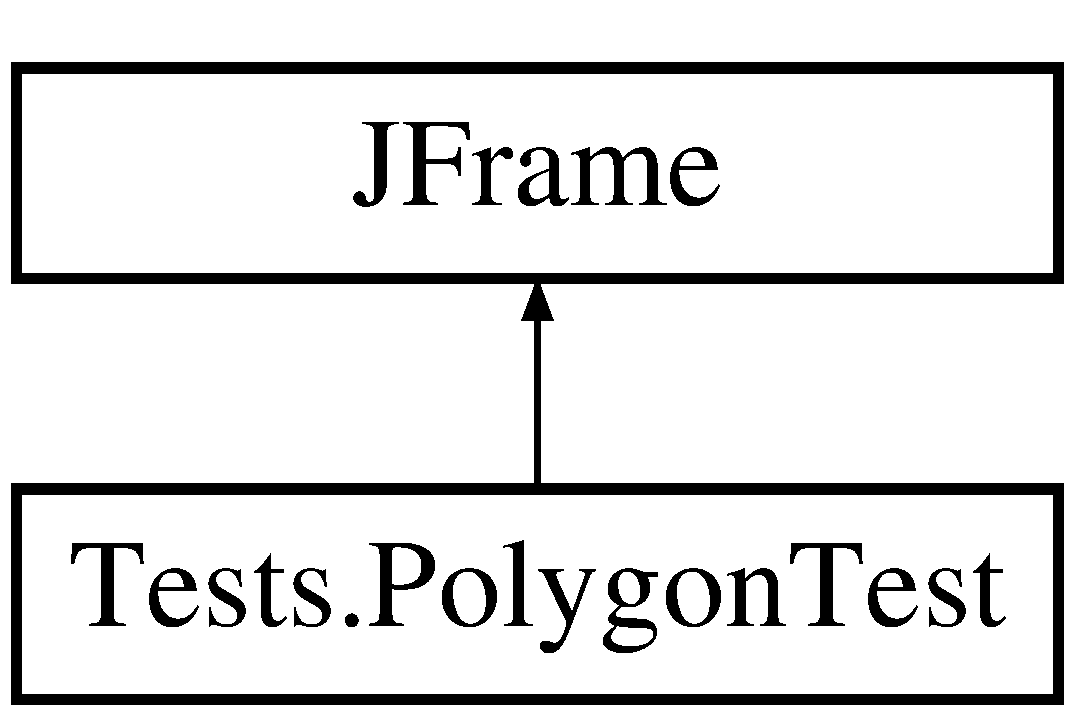
\includegraphics[height=2.000000cm]{class_tests_1_1_polygon_test}
\end{center}
\end{figure}
\subsection*{Static Public Member Functions}
\begin{DoxyCompactItemize}
\item 
\mbox{\Hypertarget{class_tests_1_1_polygon_test_ad0ef742c61990ffafc1f172fed737761}\label{class_tests_1_1_polygon_test_ad0ef742c61990ffafc1f172fed737761}} 
static void {\bfseries main} (String\mbox{[}$\,$\mbox{]} args)
\end{DoxyCompactItemize}


The documentation for this class was generated from the following file\+:\begin{DoxyCompactItemize}
\item 
/\+Users/\+Charles\+B\+Swarts/eclipse-\/workspace/\+Chess\+Library/src/\+Tests/Polygon\+Test.\+java\end{DoxyCompactItemize}

\hypertarget{class_source_files_1_1_queen}{}\section{Source\+Files.\+Queen Class Reference}
\label{class_source_files_1_1_queen}\index{Source\+Files.\+Queen@{Source\+Files.\+Queen}}
Inheritance diagram for Source\+Files.\+Queen\+:\begin{figure}[H]
\begin{center}
\leavevmode
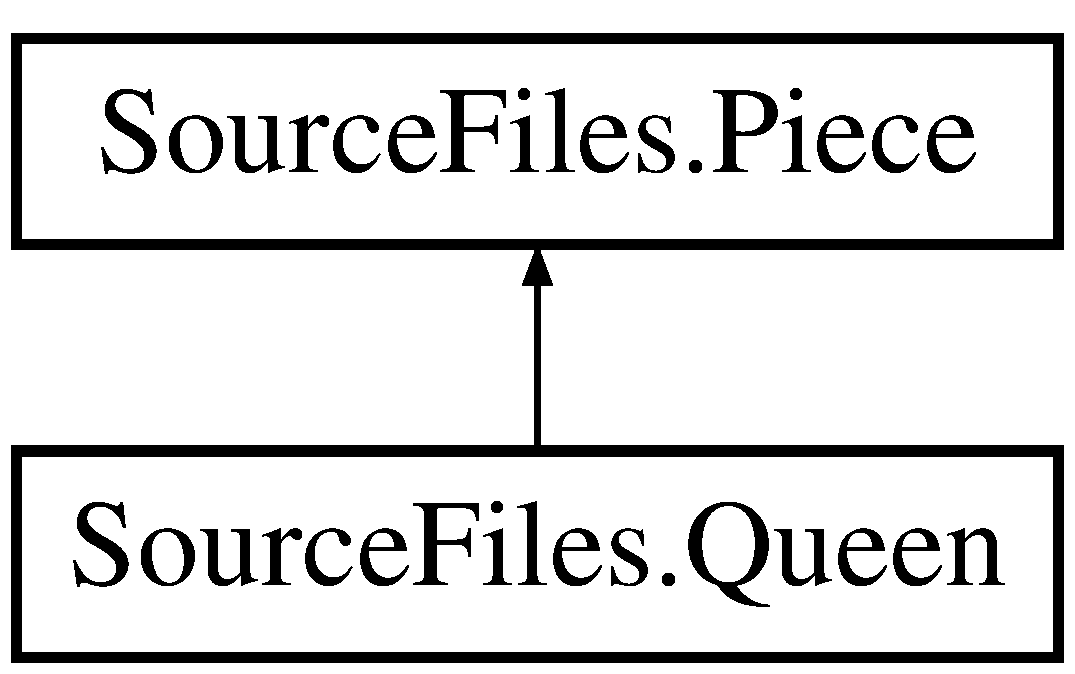
\includegraphics[height=2.000000cm]{class_source_files_1_1_queen}
\end{center}
\end{figure}
\subsection*{Public Member Functions}
\begin{DoxyCompactItemize}
\item 
\mbox{\Hypertarget{class_source_files_1_1_queen_a280d919348ba83ae68d62dd34aef847f}\label{class_source_files_1_1_queen_a280d919348ba83ae68d62dd34aef847f}} 
{\bfseries Queen} (int team)
\item 
\mbox{\Hypertarget{class_source_files_1_1_queen_a02ae5841277d331c621d09ed4ce8ba29}\label{class_source_files_1_1_queen_a02ae5841277d331c621d09ed4ce8ba29}} 
Array\+List$<$ \mbox{\hyperlink{class_source_files_1_1_coordinate}{Coordinate}} $>$ {\bfseries get\+Movement\+Path} (\mbox{\hyperlink{class_source_files_1_1_coordinate}{Coordinate}} start, \mbox{\hyperlink{class_source_files_1_1_coordinate}{Coordinate}} dest, \mbox{\hyperlink{class_source_files_1_1_field}{Field}} f)
\item 
\mbox{\Hypertarget{class_source_files_1_1_queen_ab434d2d28cd6364dc87906377f19a62c}\label{class_source_files_1_1_queen_ab434d2d28cd6364dc87906377f19a62c}} 
Array\+List$<$ \mbox{\hyperlink{class_source_files_1_1_coordinate}{Coordinate}} $>$ {\bfseries get\+All\+Possible\+Moves} (\mbox{\hyperlink{class_source_files_1_1_coordinate}{Coordinate}} start)
\item 
\mbox{\Hypertarget{class_source_files_1_1_queen_a0b7adc1b1037b63d0de7d70c87ee9f41}\label{class_source_files_1_1_queen_a0b7adc1b1037b63d0de7d70c87ee9f41}} 
Array\+List$<$ int\mbox{[}$\,$\mbox{]}$>$ {\bfseries draw\+Yourself} (int size)
\end{DoxyCompactItemize}
\subsection*{Additional Inherited Members}


The documentation for this class was generated from the following file\+:\begin{DoxyCompactItemize}
\item 
/\+Users/\+Charles\+B\+Swarts/eclipse-\/workspace/\+Chess\+Library/src/\+Source\+Files/Queen.\+java\end{DoxyCompactItemize}

\hypertarget{class_tests_1_1_queen_test}{}\section{Tests.\+Queen\+Test Class Reference}
\label{class_tests_1_1_queen_test}\index{Tests.\+Queen\+Test@{Tests.\+Queen\+Test}}
\subsection*{Public Member Functions}
\begin{DoxyCompactItemize}
\item 
\mbox{\Hypertarget{class_tests_1_1_queen_test_ab4578e6eef0448cf97f5d5393a4b4b3d}\label{class_tests_1_1_queen_test_ab4578e6eef0448cf97f5d5393a4b4b3d}} 
void {\bfseries cannot\+Move\+To\+Current\+Location\+Test} ()
\item 
\mbox{\Hypertarget{class_tests_1_1_queen_test_a4e9fa50b947a1d8824bee82a44bedd9e}\label{class_tests_1_1_queen_test_a4e9fa50b947a1d8824bee82a44bedd9e}} 
void {\bfseries move\+To\+Valid\+Locations\+Test} ()
\item 
\mbox{\Hypertarget{class_tests_1_1_queen_test_a6aeb6a4126f143f8340fd9dc1b64d0c3}\label{class_tests_1_1_queen_test_a6aeb6a4126f143f8340fd9dc1b64d0c3}} 
void {\bfseries move\+To\+Invalid\+Locations\+Test} ()
\item 
\mbox{\Hypertarget{class_tests_1_1_queen_test_a3ac906826670f0abee559f48162a3164}\label{class_tests_1_1_queen_test_a3ac906826670f0abee559f48162a3164}} 
void {\bfseries to\+The\+Right\+Test} ()
\item 
\mbox{\Hypertarget{class_tests_1_1_queen_test_a5ebf90dde5d4f17521ec5f923ad6119d}\label{class_tests_1_1_queen_test_a5ebf90dde5d4f17521ec5f923ad6119d}} 
void {\bfseries down\+To\+The\+Right\+Test} ()
\item 
\mbox{\Hypertarget{class_tests_1_1_queen_test_a820bcdf667b222caee509a8b0d2b01b6}\label{class_tests_1_1_queen_test_a820bcdf667b222caee509a8b0d2b01b6}} 
void {\bfseries to\+The\+Down\+Test} ()
\item 
\mbox{\Hypertarget{class_tests_1_1_queen_test_a828ce902c3341ed953761d3f11d56578}\label{class_tests_1_1_queen_test_a828ce902c3341ed953761d3f11d56578}} 
void {\bfseries down\+To\+The\+Left\+Test} ()
\item 
\mbox{\Hypertarget{class_tests_1_1_queen_test_a72bfcb51507a6adfb8b6891a7753d403}\label{class_tests_1_1_queen_test_a72bfcb51507a6adfb8b6891a7753d403}} 
void {\bfseries to\+The\+Left\+Test} ()
\item 
\mbox{\Hypertarget{class_tests_1_1_queen_test_a5bfeba3640366b33c6d34801fed8ec9f}\label{class_tests_1_1_queen_test_a5bfeba3640366b33c6d34801fed8ec9f}} 
void {\bfseries up\+To\+The\+Left\+Test} ()
\item 
\mbox{\Hypertarget{class_tests_1_1_queen_test_a9ac920a1318f20da88eb2c11b14a9a2b}\label{class_tests_1_1_queen_test_a9ac920a1318f20da88eb2c11b14a9a2b}} 
void {\bfseries to\+The\+Up\+Test} ()
\item 
\mbox{\Hypertarget{class_tests_1_1_queen_test_a6c4df47daf3beac90694d2cbe7b1635e}\label{class_tests_1_1_queen_test_a6c4df47daf3beac90694d2cbe7b1635e}} 
void {\bfseries up\+To\+The\+Right\+Test} ()
\end{DoxyCompactItemize}


The documentation for this class was generated from the following file\+:\begin{DoxyCompactItemize}
\item 
/\+Users/\+Charles\+B\+Swarts/eclipse-\/workspace/\+Chess\+Library/src/\+Tests/Queen\+Test.\+java\end{DoxyCompactItemize}

\hypertarget{class_source_files_1_1_rook}{}\section{Source\+Files.\+Rook Class Reference}
\label{class_source_files_1_1_rook}\index{Source\+Files.\+Rook@{Source\+Files.\+Rook}}
Inheritance diagram for Source\+Files.\+Rook\+:\begin{figure}[H]
\begin{center}
\leavevmode
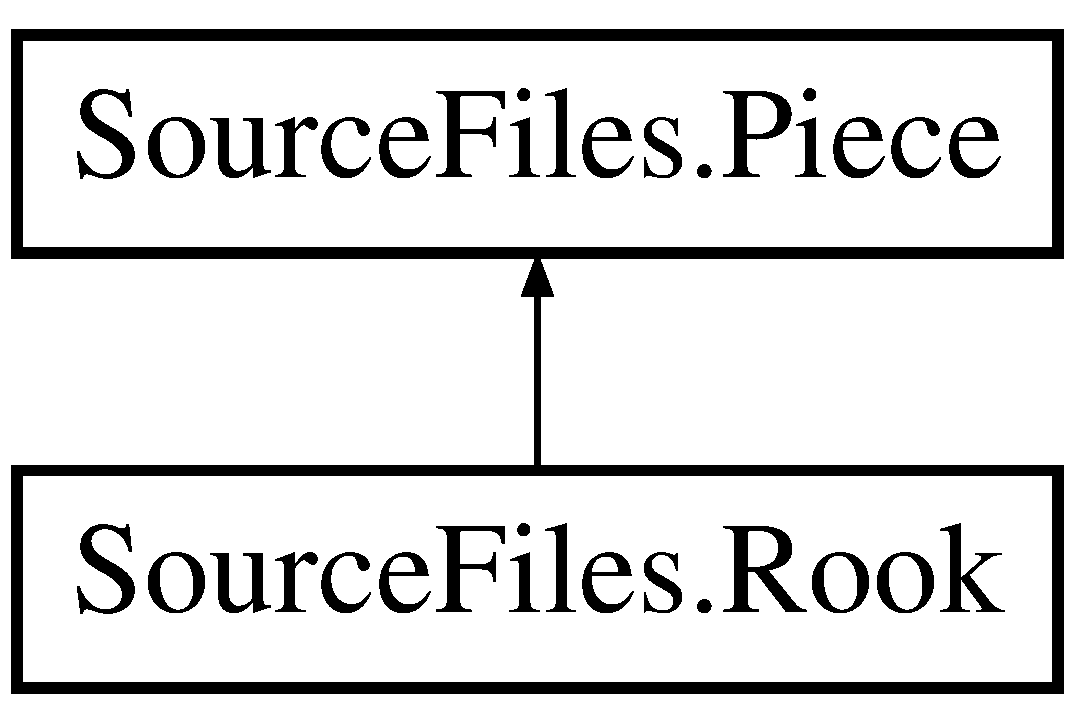
\includegraphics[height=2.000000cm]{class_source_files_1_1_rook}
\end{center}
\end{figure}
\subsection*{Public Member Functions}
\begin{DoxyCompactItemize}
\item 
\mbox{\Hypertarget{class_source_files_1_1_rook_afc515933b4b8ad359b6363b76f1ba6d6}\label{class_source_files_1_1_rook_afc515933b4b8ad359b6363b76f1ba6d6}} 
{\bfseries Rook} (int team)
\item 
\mbox{\Hypertarget{class_source_files_1_1_rook_a722958ed6f33d35198eff8c66ed0d59e}\label{class_source_files_1_1_rook_a722958ed6f33d35198eff8c66ed0d59e}} 
Array\+List$<$ \mbox{\hyperlink{class_source_files_1_1_coordinate}{Coordinate}} $>$ {\bfseries get\+Movement\+Path} (\mbox{\hyperlink{class_source_files_1_1_coordinate}{Coordinate}} start, \mbox{\hyperlink{class_source_files_1_1_coordinate}{Coordinate}} dest, \mbox{\hyperlink{class_source_files_1_1_field}{Field}} f)
\item 
\mbox{\Hypertarget{class_source_files_1_1_rook_a8e3f20050ea9209eb170e45d17e82745}\label{class_source_files_1_1_rook_a8e3f20050ea9209eb170e45d17e82745}} 
Array\+List$<$ \mbox{\hyperlink{class_source_files_1_1_coordinate}{Coordinate}} $>$ {\bfseries get\+All\+Possible\+Moves} (\mbox{\hyperlink{class_source_files_1_1_coordinate}{Coordinate}} start)
\item 
\mbox{\Hypertarget{class_source_files_1_1_rook_a88f72a165636f7a1b1af4d52b559d161}\label{class_source_files_1_1_rook_a88f72a165636f7a1b1af4d52b559d161}} 
Array\+List$<$ int\mbox{[}$\,$\mbox{]}$>$ {\bfseries draw\+Yourself} (int size)
\end{DoxyCompactItemize}
\subsection*{Additional Inherited Members}


The documentation for this class was generated from the following file\+:\begin{DoxyCompactItemize}
\item 
/\+Users/\+Charles\+B\+Swarts/eclipse-\/workspace/\+Chess\+Library/src/\+Source\+Files/Rook.\+java\end{DoxyCompactItemize}

\hypertarget{class_tests_1_1_rook_test}{}\section{Tests.\+Rook\+Test Class Reference}
\label{class_tests_1_1_rook_test}\index{Tests.\+Rook\+Test@{Tests.\+Rook\+Test}}
\subsection*{Public Member Functions}
\begin{DoxyCompactItemize}
\item 
\mbox{\Hypertarget{class_tests_1_1_rook_test_a81223434aac0b2ae7c8a45041a701b7f}\label{class_tests_1_1_rook_test_a81223434aac0b2ae7c8a45041a701b7f}} 
void {\bfseries cannot\+Move\+To\+Current\+Location\+Test} ()
\item 
\mbox{\Hypertarget{class_tests_1_1_rook_test_a347f9ed2821b93a0b28dcded9803d4df}\label{class_tests_1_1_rook_test_a347f9ed2821b93a0b28dcded9803d4df}} 
void {\bfseries move\+To\+Valid\+Locations\+Test} ()
\item 
\mbox{\Hypertarget{class_tests_1_1_rook_test_a82cc6ff5beffa18e5f6555704773e1ad}\label{class_tests_1_1_rook_test_a82cc6ff5beffa18e5f6555704773e1ad}} 
void {\bfseries move\+To\+Invalid\+Locations\+Test} ()
\item 
\mbox{\Hypertarget{class_tests_1_1_rook_test_acbb43811e924babb29a1697a438998ee}\label{class_tests_1_1_rook_test_acbb43811e924babb29a1697a438998ee}} 
void {\bfseries to\+The\+Right\+Test} ()
\item 
\mbox{\Hypertarget{class_tests_1_1_rook_test_a4ce3e69a80220546f2ddb23ba5eb3e16}\label{class_tests_1_1_rook_test_a4ce3e69a80220546f2ddb23ba5eb3e16}} 
void {\bfseries to\+The\+Down\+Test} ()
\item 
\mbox{\Hypertarget{class_tests_1_1_rook_test_aa316d7576f1da7c726967f4f8b6c9a1e}\label{class_tests_1_1_rook_test_aa316d7576f1da7c726967f4f8b6c9a1e}} 
void {\bfseries to\+The\+Left\+Test} ()
\item 
\mbox{\Hypertarget{class_tests_1_1_rook_test_af7adbb22657b686c40e2eccfe2c947c5}\label{class_tests_1_1_rook_test_af7adbb22657b686c40e2eccfe2c947c5}} 
void {\bfseries to\+The\+Up\+Test} ()
\end{DoxyCompactItemize}


The documentation for this class was generated from the following file\+:\begin{DoxyCompactItemize}
\item 
/\+Users/\+Charles\+B\+Swarts/eclipse-\/workspace/\+Chess\+Library/src/\+Tests/Rook\+Test.\+java\end{DoxyCompactItemize}

%--- End generated contents ---

% Index
\backmatter
\newpage
\phantomsection
\clearemptydoublepage
\addcontentsline{toc}{chapter}{Index}
\printindex

\end{document}
